\documentclass[aspectratio=169, 14pt]{beamer}
\usepackage[utf8]{inputenc}
\usepackage{xeCJK}
\usepackage{graphicx}
\makeatletter
\newcommand*\bigcdot{\mathpalette\bigcdot@{.5}}
\newcommand*\bigcdot@[2]{\mathbin{\vcenter{\hbox{\scalebox{#2}{$\m@th#1\bullet$}}}}}
\makeatother
\usepackage{transparent}
\usepackage[ruled, lined, linesnumbered, commentsnumbered]{algorithm2e}
\usepackage{pgfplots}
\usepackage{tikz}
\usetikzlibrary{matrix,backgrounds}
\usetikzlibrary{arrows}
\usetikzlibrary {arrows.meta}
\usetikzlibrary{calc,shadows.blur,fit,positioning}
\usetikzlibrary {shapes.multipart}
\usetikzlibrary{chains}
\usetikzlibrary{er}
\usepackage{minted}
\usepackage{fontawesome5}
\usepackage{booktabs}
\usepackage{caption}
\usepackage{subcaption}
\usepackage{hyperref}
\hypersetup{
    colorlinks=true,
    linkcolor=blue,
    filecolor=magenta,      
    urlcolor=cyan,
    }
\urlstyle{same}
\usetheme{metropolis}
\metroset{block=fill}
\usecolortheme{default}
\definecolor{darkmidnightblue}{rgb}{0.0, 0.2, 0.4}
\definecolor{LightGray}{gray}{0.9}


%------------------------------------------------------------
%This block of code defines the information to appear in the
%Title page
\title[Database Principles and Applications] %optional
{数据库原理与应用}

\subtitle{存储、索引及事务}

\author[CHEN Zhongpu] % (optional)
{CHEN Zhongpu}

\institute[] % (optional)
{
  School of Computing and Artificial Intelligence \\
  \href{mailto:zpchen@swufe.edu.cn}{zpchen@swufe.edu.cn}
}

\date[] % (optional)
{SWUFE, Fall 2022}

%End of title page configuration block
%------------------------------------------------------------


%------------------------------------------------------------
%The next block of commands puts the table of contents at the 
%beginning of each section and highlights the current section:

% \AtBeginSection[]
% {
%   \begin{frame}
%     \frametitle{Table of Contents}
%     \tableofcontents[currentsection]
%   \end{frame}
% }
%------------------------------------------------------------


\begin{document}

%The next statement creates the title page.
\frame{\titlepage}

%---------------------------------------------------------
%This block of code is for the table of contents after
%the title page
% \begin{frame}
% \frametitle{Table of Contents}
% \tableofcontents
% \end{frame}
%--------------------------------------------------------
\begin{frame}
    \frametitle{复习}
    \begin{center}
        \LARGE {\faIcon{database}}
    \end{center}
    \begin{enumerate}
        \item 如何使用数据库 (SQL)
        \item 如何设计数据库
        \item \alert{如何实现数据库}
    \end{enumerate}

\end{frame}

\begin{frame}[fragile]
    \begin{center}
        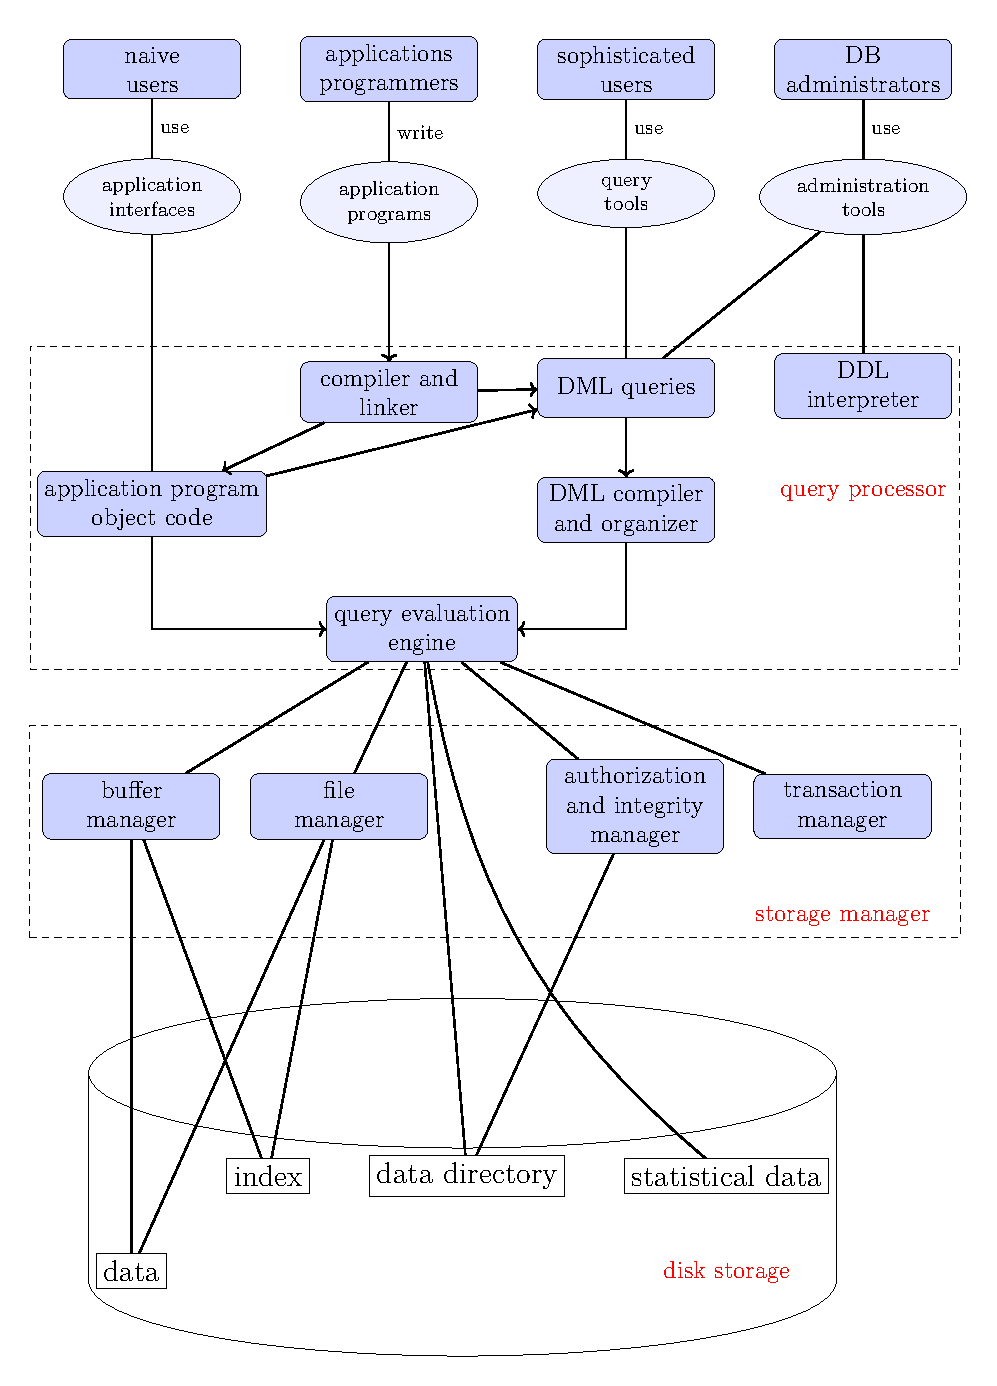
\includegraphics[height=.99\paperheight]{image/system}
    \end{center}
\end{frame}

{
    % \usebackgroundtemplate{\transparent{0.3}{\begin{picture}
    %     
\includegraphics[height=0.7\paperheight]{cover}
    % \end{picture}    
    % }}
\usebackgroundtemplate{
  \tikz[overlay,remember picture] 
  \node[opacity=0.3, at=(current page.south east),anchor=south east, yshift=2cm,xshift=4cm] {
    
\includegraphics[height=0.6\paperheight]{cover}};
}
    \begin{frame}
        \section{\textcolor{darkmidnightblue}{1. 数据库存储}}
    \end{frame}
}

\begin{frame}
    \frametitle{存储层级}

    \begin{center}
        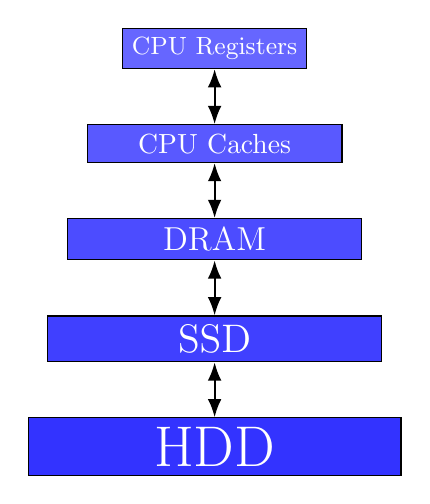
\begin{tikzpicture}[text=white]
            \node (register)[draw, fill=blue!60, ] {\small CPU Registers};
            \node (cache)[draw, fill=blue!65, below=.7cm of register, text width=3cm, align=center] {CPU Caches};
    
            \node (dram) [draw, fill=blue!70, below=.7cm of cache, text width=3.5cm, align=center]{\large DRAM};
    
            \node (ssd) [draw, fill=blue!75, below=.7cm of dram, text width=4cm, align=center]{\Large SSD};
    
            \node (hdd) [draw, fill=blue!80, below=.7cm of ssd, text width=4.5cm, align=center]{\huge HDD};


        \draw [Latex-Latex, thick] (register) -- (cache);
        \draw [Latex-Latex, thick] (dram) -- (cache);
        \draw [Latex-Latex, thick] (dram) -- (ssd);
        \draw [Latex-Latex, thick] (hdd) -- (ssd);
        \end{tikzpicture}


    \end{center}

\end{frame}

\begin{frame}
    \frametitle{背景知识}
主流数据库都是基于\alert{磁盘的}(非易失存储),在计算的时候需要从磁盘读取数据到\alert{内存}(易失存储)。
\noindent\makebox[\linewidth]{\rule{\paperwidth}{0.4pt}}
\textbf{\faIcon{question} 两个关键问题}:

\begin{itemize}
    \item 问题一:DBMS如何在磁盘中存储数据?
    \item 问题二:DBMS如何管理内存并与磁盘来回移动数据?
\end{itemize}

特别地,磁盘不适合随机访问。因此,在设计DBMS的时候,需要尽可能\textbf{连续}访问,而不是\textbf{随机}访问。
\end{frame}

\begin{frame}
    \frametitle{Latency Numbers Every Programmer Should Know}

    \begin{table}
        \begin{tabular}{lrr}
          \toprule
          L1 Cache & 1 ns & \textcolor{red}{1 sec} \\
          L2 Cache & 4 ns & \textcolor{red}{4 sec} \\
          DRAM & 100 ns & \textcolor{red}{100 sec} \\
          SSD & 16,000 ns & \textcolor{red}{4.4 hours} \\
          HDD & 2,000,000 ns & \textcolor{red}{3.3 weeks} \\
          \bottomrule
        \end{tabular}
    \end{table}
    数据来源:\href{https://colin-scott.github.io/personal_website/research/interactive_latency.html}{Latency Numbers Every Programmer Should Know}。
\end{frame}

\begin{frame}
    \frametitle{1.1 文件存储}
虽然DBMS是由传统的\alert{基于文件的处理系统}进化而来,但是DBMS还是需要使用文件来存储数据。只不过,它采用了一种自定义的格式(甚至OS也一般不知道文件的内容)。

DBMS将文件组织成一组\alert{pages}。

\begin{exampleblock}{Page}
A page is a fixed-size block of data.    
\end{exampleblock}

\end{frame}

\begin{frame}[fragile]
我们在讨论\alert{page}的时候,可能有三种语义:

\begin{itemize}
    \item 硬件page(一般是4KB)
    \item OS page(一般是4KB)
    \item DB page(4KB-16KB)
\end{itemize}
\pause
\noindent\makebox[\linewidth]{\rule{\paperwidth}{0.4pt}}
\begin{figure}
    \centering
    \begin{subfigure}[b]{0.3\textwidth}
        \centering
        
\includegraphics[width=\textwidth]{image/sqlite}
        \caption{4KB}
    \end{subfigure}
    \hfill
    \begin{subfigure}[b]{0.3\textwidth}
        \centering
        
\includegraphics[width=.6\textwidth]{image/pg}
        \caption{8KB}
    \end{subfigure}
    \hfill
    \begin{subfigure}[b]{0.3\textwidth}
        \centering
        
\includegraphics[width=\textwidth]{image/mysql}
        \caption{16KB}
    \end{subfigure}
\end{figure}

\end{frame}

\begin{frame}
    \frametitle{1.2 Page的组织}
DBMS可以使用不同的方式去组织pages:

\begin{itemize}
    \item 堆文件组织
    \item 树文件组织
    \item 顺序文件组织
    \item 哈希文件组织
\end{itemize}

\begin{tikzpicture}
    \node[fill=yellow,blur shadow={shadow xshift=-0.5ex},
    text width=26em,anchor=south west,rounded corners]
    {此时我们不需要知道page内部的内容。};
\end{tikzpicture}

\end{frame}

\begin{frame}
    \frametitle{堆文件组织(heap file organization)}

    \begin{quote}
        heap: an untidy pile or mass of things.
        \begin{flushright}
            --- Cambridge Dictionary
        \end{flushright}
    \end{quote}

    \begin{exampleblock}{Heap File}
A heap file is an unordered collection of pages/records with tuples that are stored in random order.        
    \end{exampleblock}

\faIcon{lightbulb} 思考:堆文件组织是无序的,那么如何快速找到一个page?
\end{frame}

\begin{frame}[fragile]
    \frametitle{1.3 Page的内容}
Page由header和data构成,其中\alert{header}是描述该page内容的元数据(meta-data):
\begin{columns}
    \column{.4\textwidth}
    \begin{itemize}
        \item page大小
        \item 校验和
        \item DBMS版本
        \item 压缩信息
        \item ...
    \end{itemize}
    \column{.6\textwidth}
    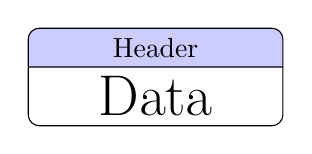
\begin{tikzpicture}[
        comment/.style={rectangle, draw=black, rounded corners,
        text centered, anchor=north, text=black, text width=3cm, minimum height=3em}, every second node part/.style={fill=white, inner ysep=4cm}]
        \node [comment, rectangle split, rectangle split parts=2, rectangle split part fill={blue!20,white}]
        {
            Header
            \nodepart{two} {\huge Data}
        };
    \end{tikzpicture}
\end{columns}

\end{frame}

\begin{frame}
    \frametitle{Page layout}
假设我们仅在page中存储元组。如果元组都是定长的,唯一的难点是\textbf{如何纪录被删除的元组},一种方案是使用\alert{free list}。

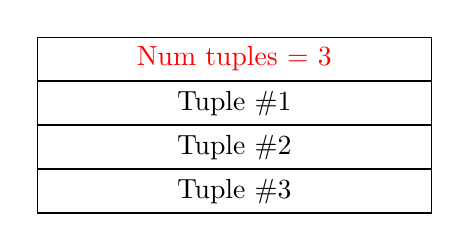
\begin{tikzpicture}[every node/.style={ minimum width=5cm}]
    \matrix [nodes=draw]
{
    \node [text=red] {Num tuples = 3 }; \\
    \node {Tuple \#1}; \\
    \node {Tuple \#2}; \\
    \node {Tuple \#3}; \\
};
\end{tikzpicture}

\faIcon{lightbulb} 思考:插入第4和第5条数据,然后再删除第2条和第4条数据,上面的page会如何变化?
\end{frame}

\begin{frame}[fragile]
    \frametitle{Page layout:变长元组}
\faIcon{check-double} 回顾:数据库中有哪些数据类型是变长的?

为了表示变长的数据,一般使用\alert{$(offset, length)$}来标记。比如,考虑大学数据库中的\texttt{instructor(10101, Srinivasan, Comp. Sci., 65000)},仅工资这个字段是定长的:

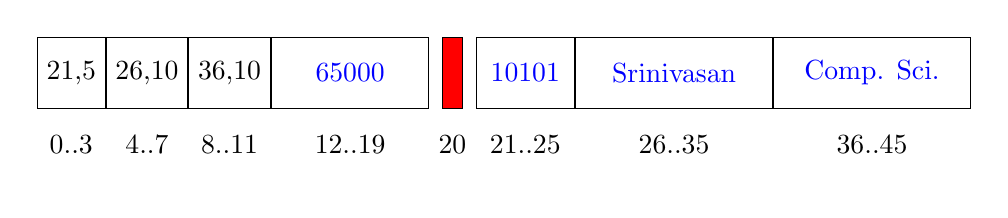
\begin{tikzpicture}
    \matrix [nodes=draw, every node/.style={minimum height=0.9cm, draw}]
{
    \node [label=below:$0..3$] {21,5}; & \node [label=below:$4..7$] {26,10}; & \node [label=below:$8..11$] {36,10}; & \node [minimum width=2cm, text=blue, label=below:$12..19$] {65000}; & \node [fill=red, minimum width=0.25cm, label=below:$20$] {}; & \node [minimum width=1.25cm, text=blue, label=below:$21..25$] {10101}; & \node [minimum width=2.5cm, text=blue, label=below:$26..35$]{Srinivasan}; & \node [minimum width=2.5cm, text=blue, label=below:$36..45$]{Comp. Sci.};  \\
};    
\end{tikzpicture}

\end{frame}

\begin{frame}[fragile]
    \frametitle{Page layout:分页的槽结构}
为了存储这些变长的元组,最常用的方式是\alert{分页的槽结构}(slotted pages),即使用一个数组(slot array)来记录每个元组的位置和大小。

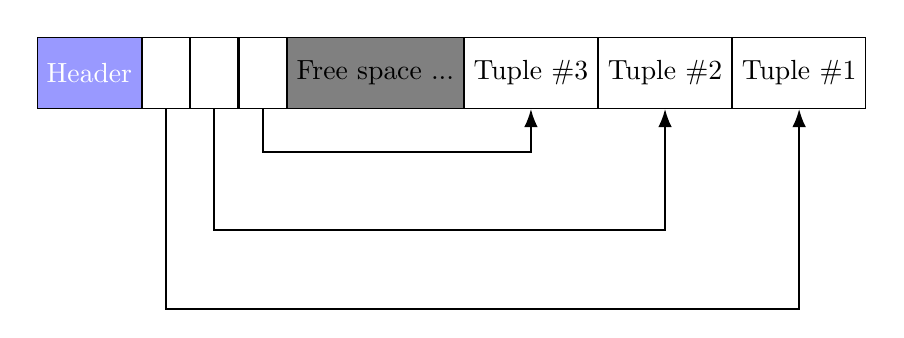
\begin{tikzpicture}
    \matrix [nodes=draw, every node/.style={minimum height=0.9cm, minimum width=.6cm, draw}]
    {
     \node [fill=blue!40, text=white] {Header}; & \node (1st) {}; & \node (2nd) {}; & \node (3rd) {}; & \node [fill=gray] {Free space ...}; & \node (3data) {Tuple \#3}; & \node (2data) {Tuple \#2}; &\node (1data) {Tuple \#1};\\   
    };    

    \draw [-Latex, thick] (1st) -- ++(0,-3) -| (1data);

    \draw [-Latex, thick] (2nd) -- ++(0,-2) -| (2data);

    \draw [-Latex, thick] (3rd) -- ++(0,-1) -| (3data);
\end{tikzpicture}
\end{frame}

\begin{frame}[fragile]
    \frametitle{1.4 存储模型}

    \begin{tikzpicture}
        \node[fill=yellow,blur shadow={shadow xshift=-0.5ex},
        text width=26em,anchor=south west,rounded corners]
        {关系模型并没有要求DBMS是否将一个元组的所有属性都存储在一个page。};
    \end{tikzpicture}

    \alert{行存储}(row-storage)也称\underline{n-ary storage model}(NSM):\textbf{DBMS将一个元组的所有属性在page内连续存储}。
    
    \alert{列存储}(column-storage)也称\underline{decomposition storage model}(DSM):\textbf{DBMS将所有元组的单个属性在page内连续存储}。

\end{frame}

\begin{frame}[fragile]

针对不同的工作负载(如OLAP,OLTP),使用不同的存储模型对性能影响很大:

\begin{minted}[bgcolor=LightGray, baselinestretch=1.1]{sql}
INSERT INTO instructor(ID, name, salary, dept_name)
VALUES('5566', 'Mike', 60000, 'Music');

SELECT * FROM instructor
WHERE ID = '5566';

SELECT COUNT(*)
FROM instructor
WHERE department = 'Music';
\end{minted}

\end{frame}

\begin{frame}[fragile]
    \frametitle{列存储的元组识别}
    \begin{itemize}
        \item 方式一:\textbf{固定长度的偏移}
        \item 方式二:\textbf{嵌入元组ID}
    \end{itemize}

    \begin{tikzpicture}
            \matrix (offset) [nodes=draw, every node/.style={minimum height=0.9cm, minimum width=.9cm, draw}, column sep=.5cm]
            {
             \node [fill=blue!40, text=white] {A}; &\node [fill=blue!40, text=white] {B}; &\node [fill=blue!40, text=white] {C}; \\ 
             \node [label=left:$0$] {}; & \node {}; &\node {}; \\ 
             \node [label=left:$1$] {}; & \node {}; &\node {}; \\
             \node [label=left:$2$]{}; & \node {}; &\node {}; \\ 
            };       
            \node [below=.1cm of offset] {方式一}; 
            
            \matrix (embed) [nodes=draw, every node/.style={minimum height=0.9cm, minimum width=1.15cm, draw}, column sep=.5cm, right=of offset]{
                \node [fill=blue!40, text=white] {A}; &\node [fill=blue!40, text=white] {B}; &\node [fill=blue!40, text=white] {C}; \\ 
                \node [rectangle split, rectangle split horizontal, rectangle split parts=2] {0
                \nodepart{two} {}
                }; & \node [rectangle split, rectangle split horizontal, rectangle split parts=2] {0
                \nodepart{two} {}
                }; & \node [rectangle split, rectangle split horizontal, rectangle split parts=2] {0
                \nodepart{two} {}
                }; \\
                \node [rectangle split, rectangle split horizontal, rectangle split parts=2] {1
                \nodepart{two} {}
                }; & \node [rectangle split, rectangle split horizontal, rectangle split parts=2] {1
                \nodepart{two} {}
                }; & \node [rectangle split, rectangle split horizontal, rectangle split parts=2] {1
                \nodepart{two} {}
                }; \\
                \node [rectangle split, rectangle split horizontal, rectangle split parts=2] {2
                \nodepart{two} {}
                }; & \node [rectangle split, rectangle split horizontal, rectangle split parts=2] {2
                \nodepart{two} {}
                }; & \node [rectangle split, rectangle split horizontal, rectangle split parts=2] {2
                \nodepart{two} {}
                }; \\
            };
            \node [below=.1cm of embed] {方式二}; 
    \end{tikzpicture}
\end{frame}


\begin{frame}[fragile]
    \frametitle{练习}
考虑关系\texttt{R(\underline{q\_id}, txns, total, failed)},所有属性都是定长且长度相同。假设R有20,000条元组,恰好存储在100个pages中,并忽略page header等元数据。如果DBMS使用列存储,那么为了回答下面的查询:

\begin{minted}[bgcolor=LightGray, baselinestretch=1]{sql}
SELECT total - failed FROM R
WHERE q_id = 96 AND txns > 420;
\end{minted}
    
DBMS需要从磁盘最少读取多少个pages?

\end{frame}

\begin{frame}
    \section{\textcolor{darkmidnightblue}{2. 索引(index)}}
    A database index is a data structure that improves the speed of data retrieval operations on a database table at the cost of additional writes and storage space to maintain the index data structure.
\end{frame}

\begin{frame}
    \begin{columns}
        \column{.5\textwidth}
        
\includegraphics[width=.8\textwidth]{week11/dict}
        \column{.5\textwidth}
        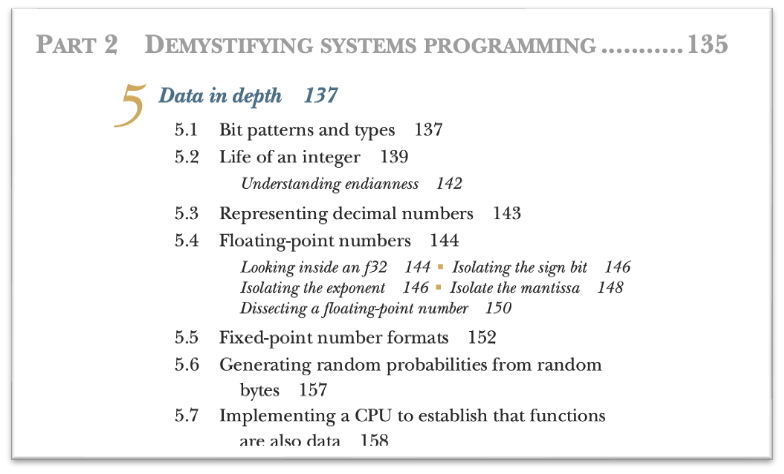
\includegraphics[width=.99\textwidth]{week11/book}
    \end{columns}
\end{frame}

\begin{frame}
    \frametitle{2.1 索引的分类}
\begin{itemize}
    \item \textbf{有序索引}(ordered index):基于值的顺序排列
    \item 哈希索引(hash index)
\end{itemize}

\noindent\makebox[\linewidth]{\rule{\paperwidth}{0.4pt}}

例子:考虑一个排序的数组$\{1, 3, 4, 8, 10, 14, 15\}$,如何快速找到key的位置?

\end{frame}

\begin{frame}
    \frametitle{2.2 有序索引:聚集 vs. 非聚集}
\begin{exampleblock}{聚集索引}
如果索引的搜索码也能决定包含文件中记录的排序: \alert{聚集索引}(clustering index)或 主索引(primary index)。    
\end{exampleblock}

\begin{table}
    \begin{tabular}{llll}
      \toprule
      ID & name & dept\_name & salary \\
      \midrule
      10101 & Srinivasan & Comp. Sci. & 65000 \\
      12121 & Wu & Finance & 9000 \\
      15151 & Mozart & Music & 40000 \\
      22222 & Einstein & Physics & 95000 \\
      \bottomrule
    \end{tabular}
\end{table}
\end{frame}

\begin{frame}
聚集索引所依赖的文件组织方式是\alert{顺序文件组织}(sequential file organization)。
\noindent\makebox[\linewidth]{\rule{\paperwidth}{0.4pt}}
如果搜索码指定的排序与文件中记录的排序不同,那么它就是非聚集索引(non-clustering index)或者辅助索引(secondary index)。

\faIcon{lightbulb} 思考:一个表能否有多个聚集索引?
\end{frame}

\begin{frame}
    \frametitle{2.3 有序索引:稠密 vs. 稀疏}
    \begin{columns}
        \column{.5\textwidth}
        毛孔(记录)、头发(索引)
        
\includegraphics[width=.99\textwidth]{week11/hair}
        \column{.5\textwidth}
        In a dense index, an index entry appears for every search-key value in the file.
    \end{columns}

\end{frame}

\begin{frame}[fragile]
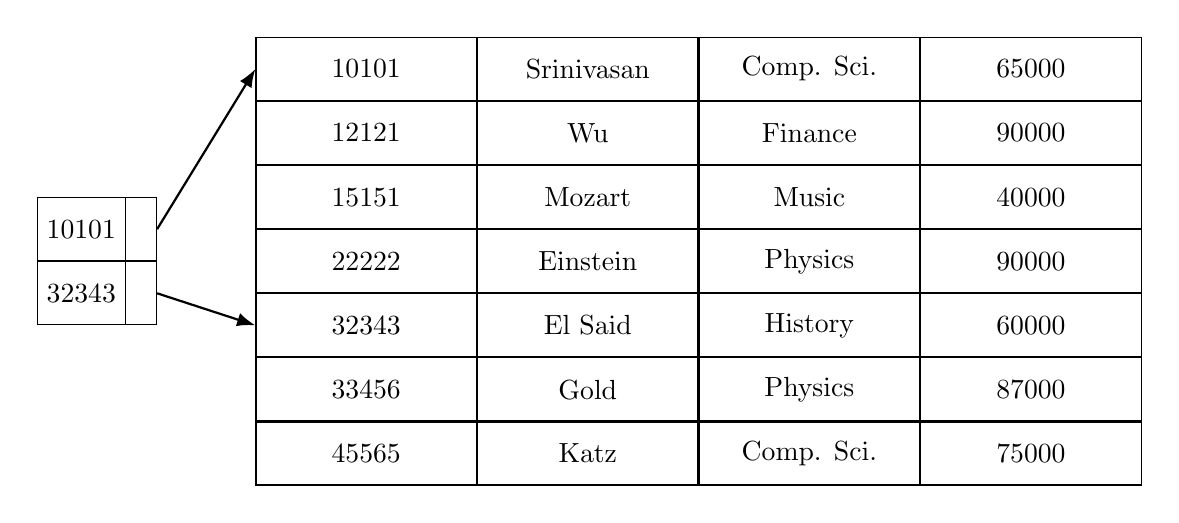
\begin{tikzpicture}
    \matrix (table) [nodes=draw, every node/.style={minimum height=0.8cm, minimum width=2.8cm, draw}] {
        \node (n10101) {10101}; & \node {Srinivasan}; & \node {Comp. Sci.}; & \node {65000}; \\
        \node {12121}; & \node {Wu}; & \node {Finance}; & \node {90000}; \\
        \node {15151}; & \node {Mozart}; & \node {Music}; & \node {40000}; \\
        \node {22222}; & \node {Einstein}; & \node {Physics}; & \node {90000}; \\
        \node (n32343) {32343}; & \node {El Said}; & \node {History}; & \node {60000}; \\
        \node {33456}; & \node {Gold}; & \node {Physics}; & \node {87000}; \\
     \node {45565}; & \node {Katz}; & \node {Comp. Sci.}; & \node {75000}; \\
    };

    \matrix [left=of table, nodes=draw, every node/.style={minimum height=0.8cm, minimum width=2cm, draw}] {
        \node [rectangle split, rectangle split horizontal, rectangle split parts=2] (i10101) {10101
                \nodepart{two} {}
                }; \\
        \node [rectangle split, rectangle split horizontal, rectangle split parts=2] (i32343) {32343
                \nodepart{two} {}
                }; \\
    };

    \draw [thick, -Latex] (i10101.east) -- (n10101.west);
    \draw [thick, -Latex] (i32343.east) -- (n32343.west);
\end{tikzpicture}

\faIcon{lightbulb} 思考:稀疏索引能否为非聚集索引?

\end{frame}

\begin{frame}[fragile]
    \frametitle{2.4 B+树索引}

    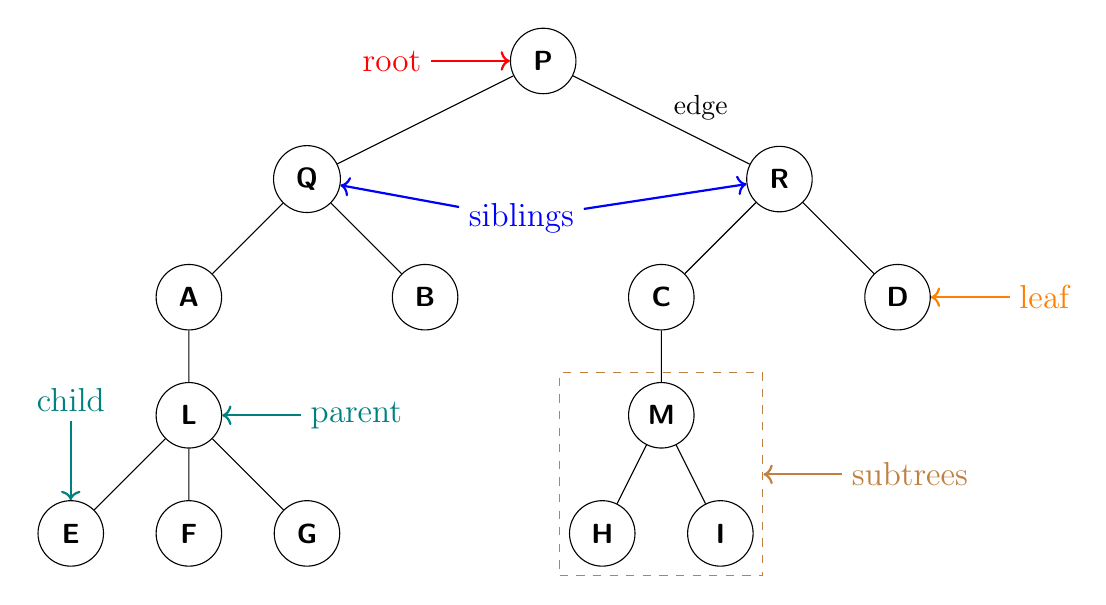
\begin{tikzpicture}[treenode/.style = {align=center, inner sep=1pt, text centered, font=\sffamily}, bst/.style = {treenode, circle, black, font=\sffamily\bfseries, draw=black, text width=2em},level/.style={sibling distance = 6cm/#1,
        level distance = 1.5cm}]
      \node [bst] (rootn) {P}
          child {node [bst](nodeq) {Q}
              child {node [bst] {A}
                child {node [bst](nodel) {L}
                  child {node [bst](nodee) {E}}
                  child {node [bst] {F}}
                  child {node [bst] {G}}
                }
              }
              child {node [bst] {B}}
          }
          child {node (noder) [bst, label={[xshift=-1.0cm, yshift=0.2cm]edge}] {R}
            child {node [bst] {C}
              child {node [bst] (nodem) {M}
                child {node [bst] (nodeh) {H}}
                child {node [bst] (nodei) {I}}
                }
            }
            child {node [bst](noded) {D}}
          }
      ;
      
      \node[left=of rootn](roott) {\large \textcolor{red}{root}};
      \draw[->, red, thick] (roott) -- (rootn);
      
      \node[right=of nodeq, yshift=-.5cm, xshift=.5cm](siblingt) {\large \textcolor{blue}{siblings}};
      
      \draw[->, blue, thick] (siblingt) -- (nodeq);
      \draw[->, blue, thick] (siblingt) -- (noder);
      
      \node[fit=(nodem)(nodei)(nodeh), dashed, draw, brown](subtrees) {};
      \node[right=of subtrees](subtreest){\large \textcolor{brown}{subtrees}};
      \draw[->, brown, thick] (subtreest) -- (subtrees);
      
      \node[right=of nodel](parentt){\large \textcolor{teal}{parent}};
      \draw[->, teal, thick] (parentt) -- (nodel);
      
      \node[above=of nodee](childt){\large \textcolor{teal}{child}};
      \draw[->, teal, thick] (childt) -- (nodee);
      
      \node[right=of noded](leaft){\large \textcolor{orange}{leaf}};
      \draw[->, orange, thick] (leaft) -- (noded);
      
      \end{tikzpicture}

\end{frame}

\begin{frame}[fragile]

    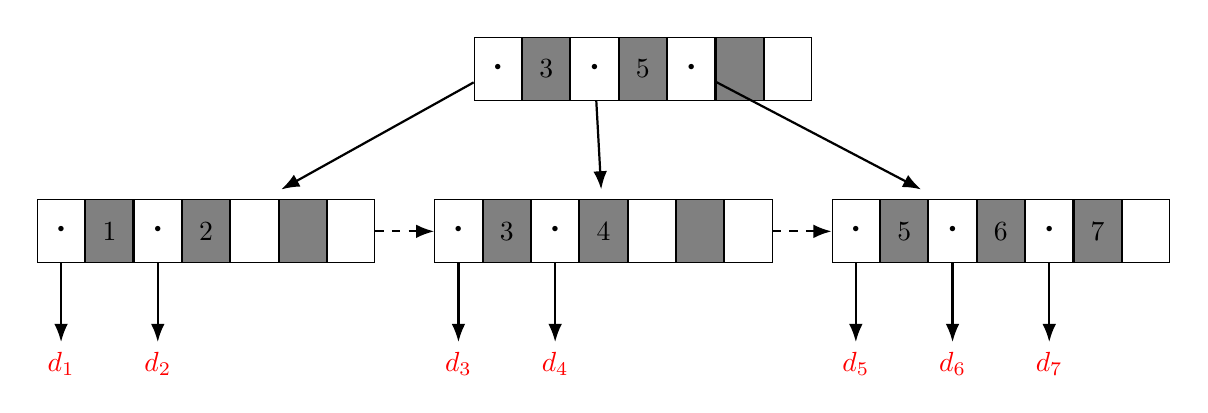
\begin{tikzpicture}
        \matrix (root) [nodes=draw, every node/.style={minimum height=0.8cm, minimum width=.6cm, draw}] {
            \node (rootp1) {$\bigcdot$}; & \node [fill=gray] {3}; & \node (rootp2) {$\bigcdot$}; & \node [fill=gray] {5}; & \node (rootp3) {$\bigcdot$}; & \node [fill=gray] {}; & \node (rootp4) {};\\
        };
        \matrix (leftnode) [nodes=draw, every node/.style={minimum height=0.8cm, minimum width=.6cm, draw}, below left=of root] {
            \node (leftnodep1) {$\bigcdot$}; & \node [fill=gray] {1}; & \node (leftnodep2) {$\bigcdot$}; & \node [fill=gray] {2}; & \node (leftnodep3) {}; & \node [fill=gray] {}; & \node (leftnodep4) {};\\
        };

        \matrix (rightnode) [nodes=draw, every node/.style={minimum height=0.8cm, minimum width=.6cm, draw}, right=.5cm of leftnode] {
            \node (rightnodep1) {$\bigcdot$}; & \node [fill=gray] {3}; & \node (rightnodep2) {$\bigcdot$}; & \node [fill=gray] {4}; & \node (rightnodep3) {}; & \node [fill=gray] {}; & \node (rightnodep4) {};\\
        };

        \matrix (right2node) [nodes=draw, every node/.style={minimum height=0.8cm, minimum width=.6cm, draw}, right=.5cm of rightnode] {
            \node (right2nodep1) {$\bigcdot$}; & \node [fill=gray] {5}; & \node (right2nodep2) {$\bigcdot$}; & \node [fill=gray] {6}; & \node (right2nodep3) {$\bigcdot$}; & \node [fill=gray] {7}; & \node (right2node4) {};\\
        };
\draw [-Latex, thick] (rootp1) -- (leftnode);

\draw [-Latex, thick] (rootp2) -- (rightnode);

\draw [-Latex, thick] (rootp3) -- (right2node);

\node (d1) [below=of leftnodep1, red] {$d_1$};
\draw [-Latex, thick] (leftnodep1) -- (d1);

\node (d2) [below=of leftnodep2, red] {$d_2$};
\draw [-Latex, thick] (leftnodep2) -- (d2);

\node (d3) [below=of rightnodep1, red] {$d_3$};
\draw [-Latex, thick] (rightnodep1) -- (d3);

\node (d4) [below=of rightnodep2, red] {$d_4$};
\draw [-Latex, thick] (rightnodep2) -- (d4);

\node (d5) [below=of right2nodep1, red] {$d_5$};
\draw [-Latex, thick] (right2nodep1) -- (d5);

\node (d6) [below=of right2nodep2, red] {$d_6$};
\draw [-Latex, thick] (right2nodep2) -- (d6);

\node (d7) [below=of right2nodep3, red] {$d_7$};
\draw [-Latex, thick] (right2nodep3) -- (d7);

\draw [-Latex, thick, dashed] (leftnodep4) -- (rightnodep1);

\draw [-Latex, thick, dashed] (rightnodep4) -- (right2nodep1);
    \end{tikzpicture}

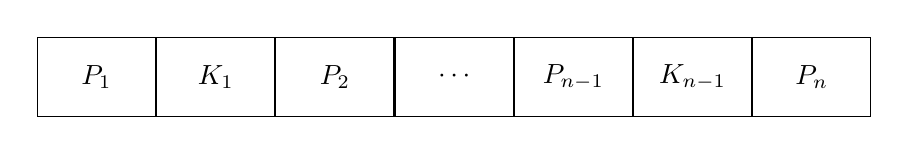
\begin{tikzpicture}
    \matrix  [nodes=draw, every node/.style={minimum height=1cm, minimum width=1.5cm, draw}, ] {
        \node {$P_1$}; & \node {$K_1$}; & \node {$P_2$}; & \node {$\cdots$}; & \node {$P_{n-1}$}; & \node {$K_{n-1}$}; & \node {$P_n$}; \\
    };
\end{tikzpicture}

\end{frame}

\begin{frame}
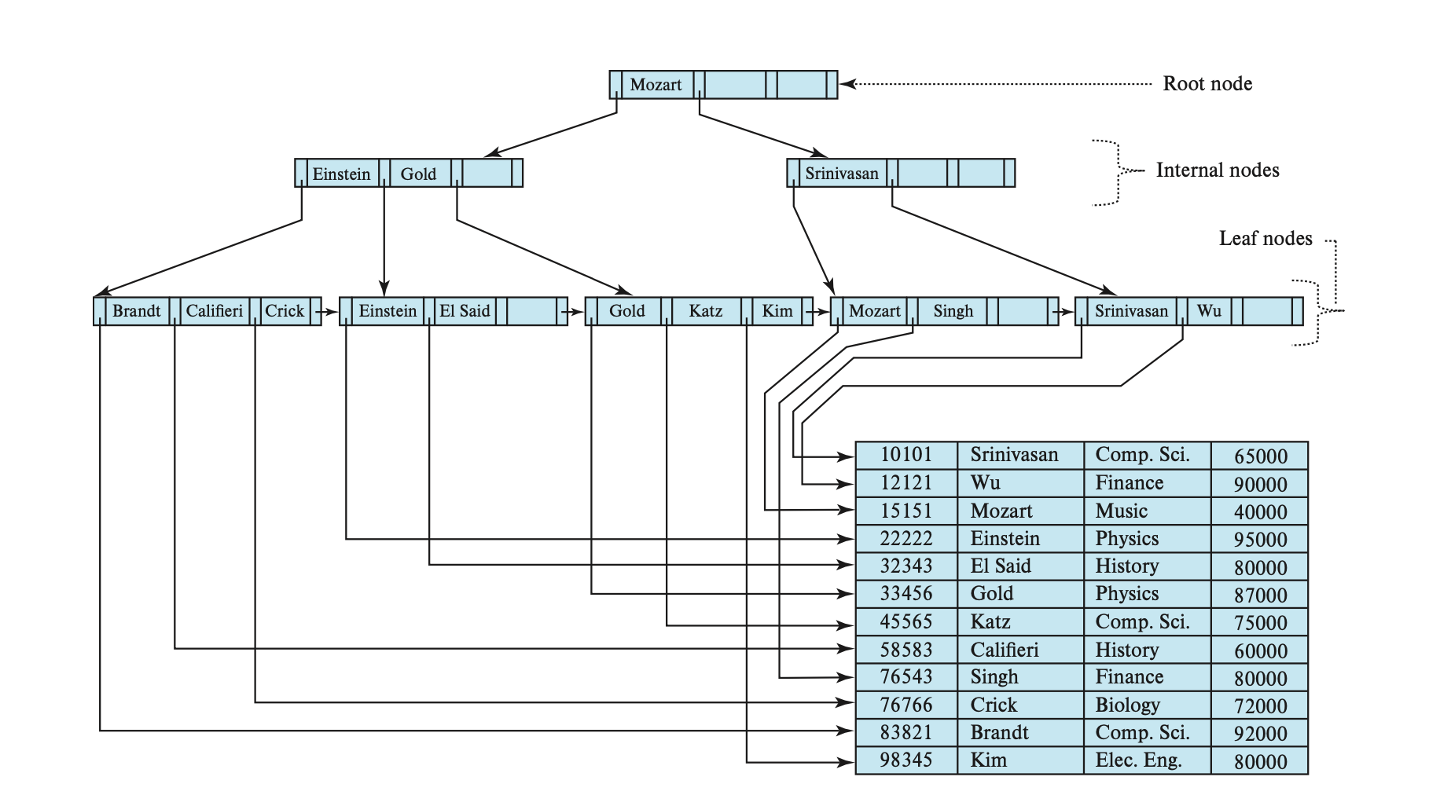
\includegraphics[width=1.1\textwidth]{week11/btree}
\end{frame}

\begin{frame}[fragile]
    \frametitle{B+树的性质}
B+树是平衡的,其高度的数量级是$\log{N}$;一个B+结点一般在一个page内(一般是4KB)。
\begin{itemize}
    \item 每个非叶子结点(除了根结点)的孩子数在n/2到n之间
    \item 根结点的孩子数在2到n之间
\end{itemize}

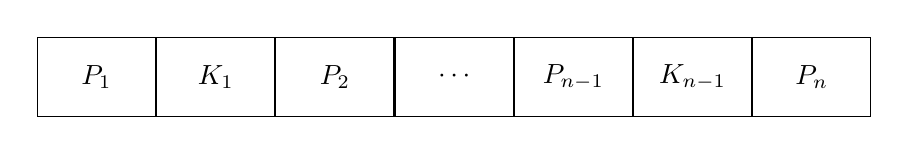
\begin{tikzpicture}
    \matrix  [nodes=draw, every node/.style={minimum height=1cm, minimum width=1.5cm, draw}, ] {
        \node {$P_1$}; & \node {$K_1$}; & \node {$P_2$}; & \node {$\cdots$}; & \node {$P_{n-1}$}; & \node {$K_{n-1}$}; & \node {$P_n$}; \\
    };
\end{tikzpicture}

\href{https://www.cs.usfca.edu/~galles/visualization/BPlusTree.html}{可视化B+树}
\end{frame}

\begin{frame}[fragile]
    \frametitle{练习}

    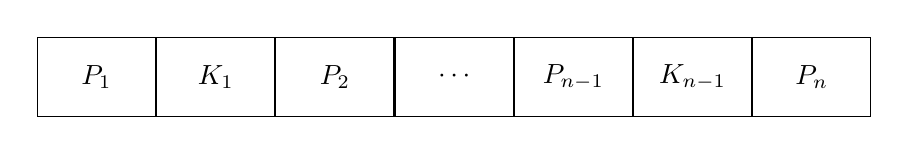
\begin{tikzpicture}
        \matrix  [nodes=draw, every node/.style={minimum height=1cm, minimum width=1.5cm, draw}, ] {
            \node {$P_1$}; & \node {$K_1$}; & \node {$P_2$}; & \node {$\cdots$}; & \node {$P_{n-1}$}; & \node {$K_{n-1}$}; & \node {$P_n$}; \\
        };
    \end{tikzpicture}

假设一个指针8 bytes,一个搜索码32 bytes,那么n大概是100。假设有1百万条记录,那么至多需要访问\rule{1cm}{0.15mm}个B+树结点。

\end{frame}

\begin{frame}[fragile]
    \frametitle{2.5 PG中的索引}
PG中主码默认会建立索引。PG仅支持非聚集索引。
    
\begin{minted}[bgcolor=LightGray]{sql} 
EXPLAIN ANALYSE 
SELECT * FROM instructor
WHERE id = '33456';

EXPLAIN ANALYSE 
SELECT * FROM instructor
WHERE name = 'Gold';
\end{minted}
\end{frame}

\begin{frame}[fragile]
    \begin{minted}[bgcolor=LightGray, baselinestretch=1]{sql} 
CREATE TABLE test_index(
    id int,
    name varchar(100)
);
INSERT INTO test_index(id, name)
    (SELECT generate_series(0, 1000000), 
    gen_random_uuid());

EXPLAIN ANALYZE SELECT * FROM test_index
WHERE id BETWEEN 100 AND 500;

CREATE INDEX id_idx ON test_index(id);
    \end{minted}
    

\end{frame}

\begin{frame}
    \frametitle{思考}
假设1个page(4KB)能够容纳100个索引项,那么对于100,000,000条元组,需要使用1,000,000个page(即4GB)来保存索引。考虑到内存的限制,应该如何做?
    

\end{frame}

\begin{frame}
    \section{\textcolor{darkmidnightblue}{3. 事务(transaction)}}
The term \alert{transaction} refers to a collection of operations that form a single logical unit of work. 
    \begin{itemize}
        \item 原子性(atomicity)
        \item 一致性(consistency)
        \item 隔离性(isolation)
        \item 持久性(durability)
    \end{itemize}

\end{frame}

\begin{frame}
    \frametitle{小结}

\begin{itemize}
    \item 存储
    \item 索引
    \item 事务
\end{itemize}

\end{frame}

\end{document}